\documentclass[a4paper, 11pt]{article}%тип документа
\usepackage{siunitx}
%отступы
\usepackage[left=2cm,right=2cm,top=2cm,bottom=3cm,bindingoffset=0cm]{geometry}
\usepackage[pdftex]{lscape}
%Русский язык
\usepackage[T2A]{fontenc} %кодировка
\usepackage[utf8]{inputenc} %кодировка исходного кода
\usepackage[english,russian]{babel} %локализация и переносы

%Вставка картинок
\usepackage{wrapfig}
\usepackage{graphicx}
\graphicspath{{Images/}}
\DeclareGraphicsExtensions{.pdf,.png,.jpg}

%Математика
\usepackage{amsmath, amsfonts, amssymb, amsthm, mathtools}

%Заголовокhttps://www.overleaf.com/project/6507f5a4176b25bf05722230
\author{Акимов М.И., Кондратюк Н.А. \\ Б06-206}

\title{Отчёт о выполнении лабораторной работы  \\ \textbf{Электрокапиллярные явления.}}
\date{\\20 марта 2024 года}
\begin{document}
 \maketitle

       \section{Цели работы.}
        \begin{itemize}
             \item Исследование базовых свойств электродов, способности поляризоваться (изменять заряд) под действием внешнего напряжения. 
             \item Знакомство с факторами, определяющими свойство поляризуемости.
             \item Знакомство с принципом работы трехэлектродной схемы, требованиям к электродам и их расположению.
             \item Исследование зависимости поверхностного натяжения на границе ртуть-раствор
             электролита от электрического потенциала.
             \item Определение потенциала нулевого заряда и емкости двойного электрического
             слоя на поверхности ртутного электрода в растворе; оценка параметров плотной
             части ДЭС.
             \item Исследование влияния природы электролита на потенциал нулевого заряда и
             величину максимального натяжения.
        \end{itemize}

        \section{Задачи работы.}
        \begin{itemize}
             \item Ознакомиться с содержанием работы; разобраться с работой потенциостата и соответствующего ПО.
             \item Провести измерения поверхностного натяжения на ртутном электроде для построения ЭК кривой. 
             \item Исходя из аппроксимаций полиномами, произвести расчёт ПНЗ, величины удельной электроёмкости и толщины ДЭС; сделать теоретический расчёт этих величин.
             \item Изучить свойства ртутного электрода, снять соответствующую ЦВАХ; провести обработку ртутного электрода в растворе фторида натрия с изучением полученных ЦВАХ.
             \item Сделать выводы о соответствии результатов реальности; сделать выводы о работе в целом; сдать и оформить отчёт о выполнении лабораторной работы.
        \end{itemize}
        \newpage
\section{Теоретическое введение.}
\subsection{Электрокапиллярные явления.} \;

\begin{wrapfigure}{l}{0.26\textwidth}
    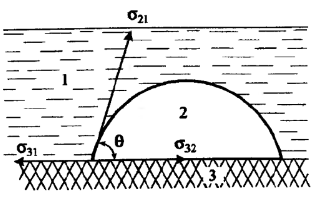
\includegraphics[width=0.26\textwidth]{Images/Уравнение Юнга.png}
    \caption{Поверхностное натяжение на границе трёх фаз.}
\end{wrapfigure}\;


\par Суть электрокапиллярных явлений заключается в изменении межфазного натяжения на поверхности раздела в результате ее заряжения (за счёт взаимного отталкивания одинаково заряженных частиц обратимая работа по увеличению поверхности раздела фаз на единицу уменьшается). При постоянном составе
электролита зависимость натяжения $\sigma$ от разности потенциалов $E$ определяется (первым) уравнением Липпмана (следует из уравнения Гиббса):
\begin{equation*}
    q = - \left(\frac{\partial \sigma}{\partial E}\right)
    \eqno(1)
\end{equation*}
\par Очевидно, что максимальное натяжение соответствует потенциалу, при котором поверхность электрода не заряжена, так называемому потенциалу нулевого заряда.
\par Из того же уравнения Гиббса следует и второе уравнение Липпмана:
\begin{equation*}
    C = - \left(\frac{\partial^2 \sigma}{\partial E^2}\right)
    \eqno(2)
\end{equation*}
\par В рамках простейшей модели Гельмгольца емкость двойного электрического слоя не зависит от разности потенциала (выполняется при высоких концентрациях
электролита и/или вдали от потенциала нулевого заряда), поэтому ЭК кривая имеет вид параболы:



\begin{equation*}
    \sigma = \sigma_0 - \frac{C}{2}(E - E_0)^2
    \eqno(3)
\end{equation*}



\par В работе производится исследование ЭК явлений на основе ртутного электрода и неполярной органической жидкости, нерастворимой в воде (деканом). В частности, применяется уравнение Юнга:



\begin{equation*}
    \sigma_{31} = \sigma_{32} + \sigma_{21} \cdot \cos{\theta}
    \eqno(4)
\end{equation*}



\par При создании разности потенциалов между ртутью и водным раствором на этой
межфазной границе возникает двойной электрический слой и межфазное натяжение
$\sigma_{31}$ меняется в соответствии с уравнением Липпмана при изменении разности потенциалов. На других межфазных границах натяжение практически не меняется. Это и позволяет исследовать изменение поверхностного натяжения на границе раздела ртутный электрод-раствор электролита в зависимости от потенциала электрода с помощью измерения краевого угла смачивания органической жидкости $\theta$.

\subsection{Поляризуемые и неполяризуемые электроды.}\;
\par Поляризация электрода - изменение потенциала под действием эликтрического тока. Электрический ток
может быть связан с протеканием окислительно-восстановительного процесса (фарадеевский ток) на электроде, либо с заряжением двойного электрического слоя (ток заряжения). Для наглядного понимания этих различий существует схема Эршлера-Рэндлса. 

Величина фарадеевского сопротивления $\Theta$ обусловлена величиной энергетического барьера электрохимической реакции (как энергия активации для химических реакций). Для протекания тока и преодоления этого барьера необходимо прикладывать к электроду определённую величину перенапряжения. Если же $\Theta$ велико, то весь ток идёт на заряжение ёмкости ДЭС и электрическая схема представляется в виде параллельно соединённых конденсатора и резистора. В этом идеальном случае электрод называется идеально поляризуемым. В реальности с ростом заряда и потенциала электрода ток электрохимической реакции постепенно усиливается  и начинает преобладать над током заряжения. Поэтому абсолютно идеально поляризуемых электродов нет и можно говорить лишь об интервале разности потенциалов, в котором электрод можно считать поляризуемым.

Обратной ситуацией являются идеально неполяризуемые электроды с очень низким $\Theta$. Зарядить их поверхность с помощью внешнего источника напряжения практически невозможно, так как в ответ на такую попытку возникает электрический ток, сбрасывающий «лишний» заряд, оставляя потенциал практически неизменным (изменить потенциал электрода можно только в соответствии с уравнением Нернста). Типичными представителями обратимых идеально неполяризуемых электродов являются все электроды сравнения. 


\section{Ход работы.}
\subsection{Исследование электрокапиллярной кривой на ртути.} \;
\par Проведём изучение ЭК кривой на ртутном электроде с помощью измерения краевого угла смачивания декана на поверхности электрода в водном растворе $0,1$ M NaF.
\par Для измерений будем использовать следующую трёхэлектродную схему: соединённые контакты $\;$"Work"$\;$ и $\;$"Comp"$\;$ подключены к проволоке, опущенной в слой ртути на дне кюветы; контакт $\;$"Counter"$\;$ подключен к Pt противоэлектроду; контакт $\;$"Ref"$\;$ к хлорсеребряному электроду сравнения.
\par Нанесём $\sim 10$ мкл декана на поверхность ртути и, варьируя подаваемый на электрод потенциал, с помощью камеры задетектируем наличие капли на поверхности электрода. Предварительно проведём тренировку капли. Для этого будем изменять потенциал ртутного электрода в диапазоне от $300$ до $ -1300$ мВ относительно электрода сравнения в циклическом режиме со скоростью развертки около $50$ мВ/с. 
\begin{table}[h!]
\centering
\caption{Данные для построения ЭК кривой.}
\begin{tabular}{|l|l|l|l|}
\hline
$E$, мВ & theta E, $^\circ$ & $\theta, ^\circ$ & $\sigma,$ мН/м      \\ \hline
300     & 107,2/107,8/108,0 & 72,8/72,2/72,0   & 390,08/390,59/390,76\\ \hline
200     & 109,0/109,3/112,0 & 71,0/70,7/68,0   & 391,60/391,86/394,10\\ \hline
100     & 121,0/122,8/126,0 & 59,0/57,2/54,0   & 401,27/402,63/404,98\\ \hline
0       & 133,8/134,7/135,8 & 46,2/45,3/44,2   & 410,30/410,87/411,56\\ \hline
-100    & 139,0/140,6/143,5 & 41,0/39,4/36,5   & 413,49/414,41/416.00\\ \hline
-200    & 151,2/153,8/154,2 & 28,8/26,2/25,8   & 419,69/420,76/420,92\\ \hline
-300    & 158,8/158,1/159,4 & 21,2/21,9/20,6   & 422,55/422,32/422,74\\ \hline
-400    & 158,1/161,5/163,0 & 21,9/18,5/17,0   & 422,32/423,36/423,77\\ \hline
-500    & 163,4/161,9/160,3 & 16,6/18,1/19,7   & 423,87/423,48/423,01\\ \hline
-600    & 163,0/162,9/163,6 & 17,0/17,1/16,4   & 423,77/423,75/423,93\\ \hline
-700    & 160,2/161,8/161,3 & 19,8/18,2/18,7   & 422,98/423,45/423,31\\ \hline
-800    & 151,1/149,9/147,7 & 28,9/30,1/32,3   & 419,65/419,12/418,11\\ \hline
-900    & 144,1/142,8/143,6 & 35,9/37,2/36,4   & 416,31/415,62/416,05\\ \hline
-1000   & 137,0/136,9/135,8 & 43,0/43,1/44,2   & 412,30/412,24/411,56\\ \hline
-1100   & 122,4/119,8/122,5 & 57,6/60,2/57,5   & 402,33/400,35/402,40\\ \hline
-1200   & 100,8/103,2/103,4 & 79,2/76,8/76,6   & 384,56/386,65/386,82\\ \hline
-1300   & 67,2/65,6/64,0    & 112,8/114,4/116,0& 355,24/353,93/352,64\\ \hline
\end{tabular}
\end{table}
\par Проведём измерения краевого угла капли при разных потенциалах (в диапазоне от $300$ до $ -1300$ мВ). Делать это будем с помощью фотографий капли декана и программы ImageJ. Поверхностное натяжение на границе ртуть/раствор будем рассчитывать по следующей формуле:
$$\sigma_\text{Hg/solution} = \sigma_\text{Hg/decane} + \sigma_\text{decane/solution}\cdot \cos(\theta)$$
\par Так как программа ImageJ проводит измерение угла, смежного с краевым, с помощью аппроксимации эллипсом, то необходимо будет учитывать этот факт при расчётах. Также для увеличения точности дальнейших вычислений будем проводить до трёх измерений на одной фотографии при данном потенциале. Все, необходимые величины отражены в Таблице 1.

\par По приведённым данным построим ЭК кривую, представленную на Рис. 2. 
\par Для определения потенциала нулевого заряда (ПНЗ) и ёмкости двойного электрического слоя воспользуемся аппроксимациями полученных точек полиномами 2-ой и 4-ой степени. 
    \begin{figure}[h!]
	\centering{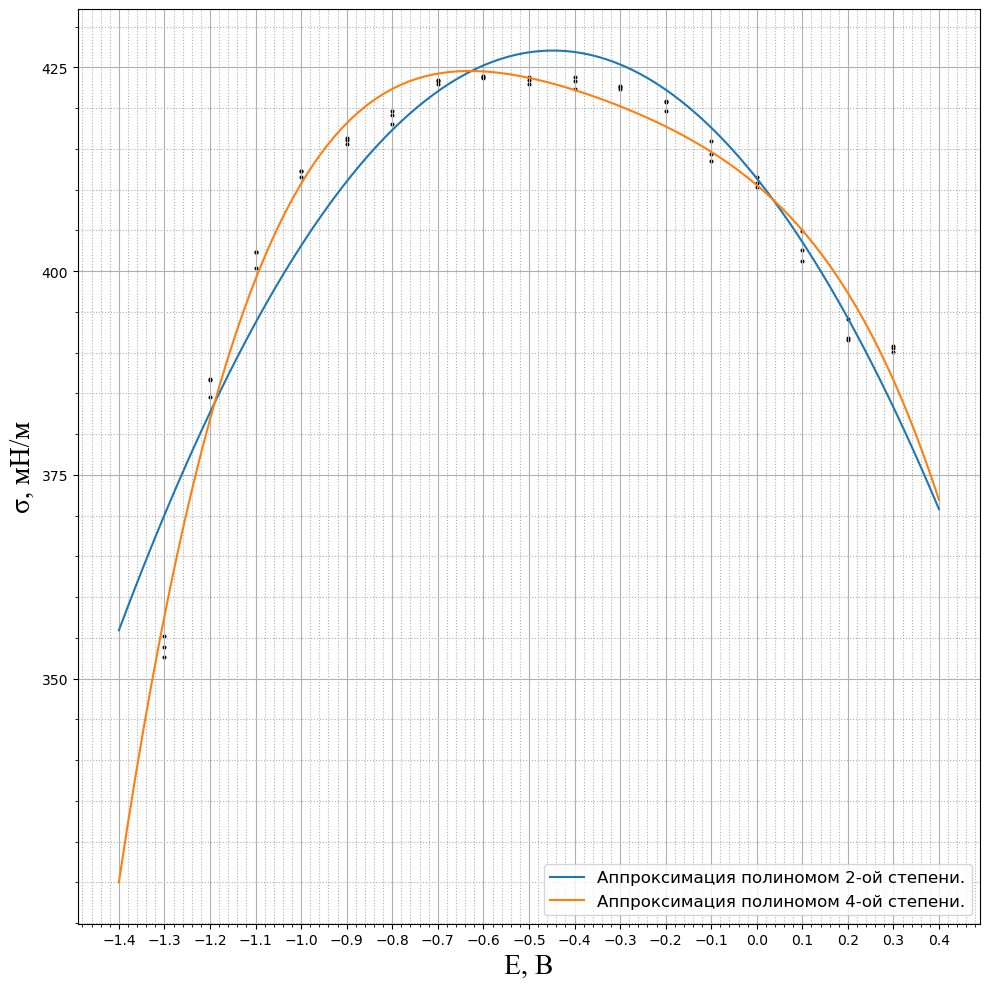
\includegraphics [scale=0.52]{Images/ЭК1.png}}
        \caption{Электрокапиллярная кривая ртутного электрода.}
    \end{figure} \;
\par Используя 1-ое уравнение Липпмана (1), найдём ПНЗ для каждой аппроксимации:
$$\text{Полученный полином 2-ой степени:} \;y = -78,39\cdot x^2 -70,13\cdot x + 411,39$$
$$\text{Полученный полином 4-ой степени:} \;y = -72,54\cdot x^4 -98,23\cdot x^3 -72,67\cdot x^2 -47,16\cdot x + 410,57$$
$\text{Условия уравнения Липпмана:}$
$$0 = -156,78\cdot x - 70,13$$
$$0 = -290,16\cdot x^3 -294,69\cdot x^2 - 145,34\cdot x -47,16$$
\par В итоге, получаем следующие значения ПНЗ:
$$E_{2, \text{ПНЗ}} = -447,32 \; \text{мВ}$$
$$E_{4, \text{ПНЗ}} = -630,04 \; \text{мВ}$$
\par Оценить на сколько данные значения соответсвуют действительности не предсталяется возможным, так как в большинстве справочников данная величина указана относительно либо водородного электрода сравнения, либо каломельного. Можем лишь визуально сказать, что аппроксимация полиномом второй степени более точная, чем 4-ой. При этом, так же из первого уравнения Липпмана (2) отметим, что при сдвиге потенциала относительно ПНЗ вправо по горизонтальной оси на электроде адсорбируются катионы, в противном случае - анионы. 
\par Тем не менее, из полученных аппроксимаций всё-таки можно сделать выводы об их корректности. Произведём оценку ёмкости двойного электрического слоя (ДЭС) вблизи ПНЗ по второму уравнению Липпмана (2):
$$C_{2, \text{ПНЗ}} = -\left(\frac{\partial^2 \sigma}{\partial x^2}\right)_{c} = 15,68 \; \text{мкФ}/\text{см}^2$$
$$C_{4, \text{ПНЗ}} = -\left(\frac{\partial^2 \sigma}{\partial x^2}\right)_{c} = 11,95 \; \text{мкФ}/\text{см}^2$$
\par Оценим для начала ёмкость ДЭС, исходя из теории Гуи-Чапмена (впоследствии будет понятно, почему). Для этого воспользуемся теоретическим соотношением электроёмкости ДЭС при ПНЗ:
$$C_{\text{Г-Ч}} = \sqrt{\frac{2 \varepsilon \varepsilon_0 F^2 c}{RT}} \approx 73,89 \; \text{мкФ}/\text{см}^2 $$
\par Отсюда можно уже с уверенностью говорить о том, что модель Гуи-Чапмена не применима для данных условий. Следовательно, для эксперимента более применима теория Гельмгольца. Этот же вывод следует и из теории Штерна, которая применима всегда:
$$\frac{1}{C} = \frac{1}{C_{\text{Г-Ч}}} + \frac{1}{C_{\text{Г}}}$$
\par Из рассчётов следует, что при высоких концентрациях ёмкость почти совпадает с гельмгольцевской. Тем не менее, по полученным данным на всякий случай оценим толщину диффузного слоя:
$$R_{\text{Д}} = \frac{\varepsilon \varepsilon_0}{C_{\text{Г-Ч}}} = 9,7 \; \si{\angstrom}$$
\par Вернёмся к модели Гельмогольца. Основная проблема, связанная с рассчетами в данной теории, - отличие диэлектрической проницаемости молекул воды в плотном слое. Для начала примем её $\varepsilon =  4 \div 6$. Исходя из данного приближения, посчитаем толщину ДЭС по Гельмгольцу:
$$ 2,26 \; \si{\angstrom} \leq d_2 \leq 3,39 \; \si{\angstrom}$$
$$ 2,96 \; \si{\angstrom} \leq d_4 \leq 4,44 \; \si{\angstrom}$$

\par Так как в теории Гельмгольца толщина ДЭС определяется радиусами гидратированных ионов, оценим их из предельных электропроводностей фторид-ионов и натрий-ионов:
$$r_{Na} = \frac{e F}{6 \pi \eta \lambda_{0,Na} } = 1,63 \; \si{\angstrom}$$
$$r_{F} = \frac{e F}{6 \pi \eta \lambda_{0,F} } = 1,48 \; \si{\angstrom}$$

\par Отметим, что порядок величины верный, но числа всё-таки отличаются. 
\par Попробуем произвести пересчёт толщины ДЭС, используя модель Штерна:
$$C_{2, \text{Г}} = 19,90 \; \text{мкФ}/\text{см}^2$$
$$C_{4, \text{Г}} = 14,26 \; \text{мкФ}/\text{см}^2$$
\par Тогда получаем следующие диапазоны толщины ДЭС:
$$1,78 \; \si{\angstrom} \leq d_2 \leq 2,67 \; \si{\angstrom}$$
$$2,48 \; \si{\angstrom} \leq d_4 \leq 3,72 \; \si{\angstrom}$$
\par Таким образом, получены значения, отвечающие посчитанным из табличных (для аппроксимации 4-ой степени хуже). В итоге, можно говорить о хорошей применимости ЭК методов для изучения ДЭС. 
\subsection{Исследование поляризуемости ртутного электрода в растворе NaF.}\;
\par Будем проводить дальнейшие измерения так же в 0,1М растворе NaF. Для начала снимем циклическую вольт-амперную характеристику (ЦВАХ) Hg электрода относительно хлорсеребряного электрода (ХСЭ) от -2100 до 300 мВ (Рис. 3). График соответствует поляризуемому электроду с областью поляризации от -1,7 до 0 В.

    \begin{figure}[h!]
	\centering{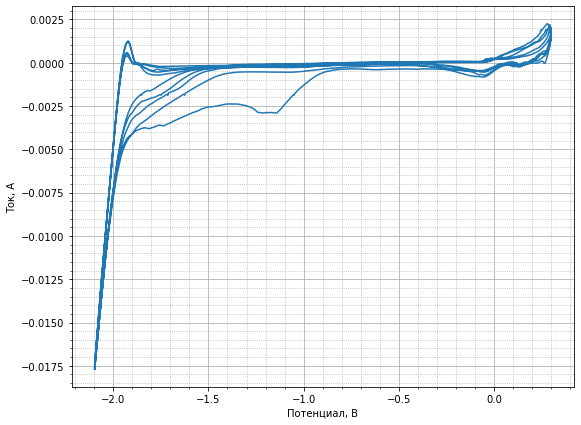
\includegraphics [scale=0.7]{Images/цвах1.png}}
        \caption{ЦВАХ Hg электрода до обработки.}
    \end{figure} \;
\par Проведём обработку Hg электрода при -2300 мВ относительно ХСЭ в течение 3 минут. За это время Na будет восстанавливаться на ртути и растворяться в ней, образуя амальгаму.
\[ Na^+ + e^- = Na_{(Hg)}\]
\par После обработки при небольших отклонениях от потенциала разрыва цепи (ПРЦ) (-2010 мВ) Hg электрод ведёт себя как неполяризуемый электрод: ток линейно зависит от приложенного напряжения в области от -2,2 В до -1,8 В (Рис. 4).
 \begin{figure}[h!]
	\centering{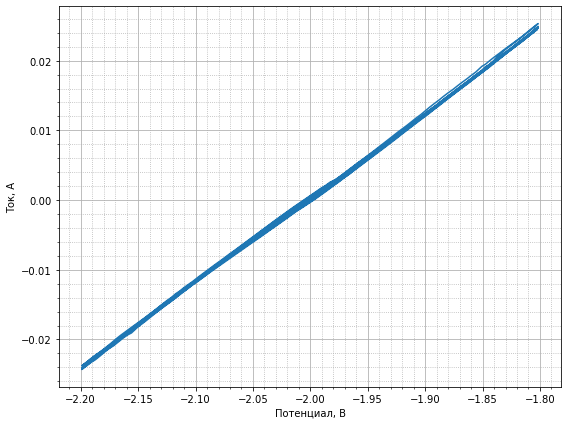
\includegraphics [scale=0.7]{Images/цвах2.png}}
        \caption{ЦВАХ Hg электрода после обработки при малых отклонениях от ПРЦ.}
    \end{figure} \;

\begin{figure}[h!]
	\centering{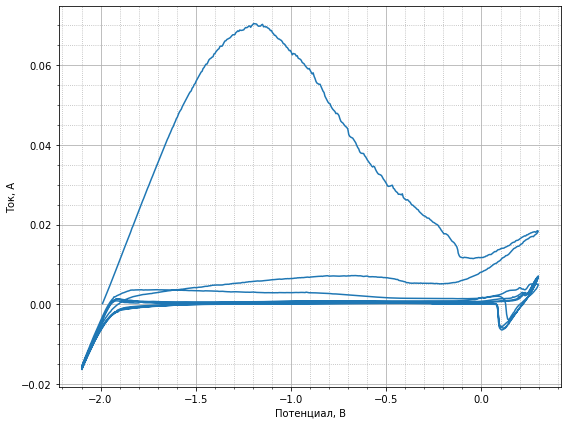
\includegraphics [scale=0.7]{Images/цвах3.png}}
        \caption{ЦВАХ Hg электрода после обработки при больших отклонениях от ПРЦ.}
\end{figure} \;
\par Однако при большем увеличении потенциала (до -1,25 В) график ЦВАХ загибается (Рис. 5), так как Na начинает выходить из ртути и окисляется в реакции с водой, наблюдается активное выделение молекулярного водорода.
\[ 2Na_{Hg} + 2H_2O = 2NaOH + H_2 \uparrow\]
\par Когда Hg электрод окончательно очистился от Na - график ЦВАХ возвращается к характеристикам поляризуемого Hg электрода.
\section{Выводы.} \;
\par Первая часть работы подразумевает построение ЭК кривой по измерениям краевого угла на границе раздела трёх фаз (ртуть/раствор/декан) при разных потенциалах. Полученные точки были аппроксимированы полиномами 2-ой и 4-ой степени. Из аппроксимирующих уравнений получены значения ПНЗ: $E_{2, \text{ПНЗ}} = -447,32 \; \text{мВ}, \; E_{4, \text{ПНЗ}} = -630,04 \; \text{мВ}$. Используя второе уравнение Липпмана по тем же уравнениям были посчитаны удельные электроёмкости ДЭС и с помощью теории Штерна оценены величины соответствующих гельмгольцовских удельных электроёмкостей: $C_{2, \text{Г}} = 19,90 \; \text{мкФ}/\text{см}^2, \; C_{4, \text{Г}} = 14,26 \; \text{мкФ}/\text{см}^2$. Наконец, по гельмгольцевским электроёмкостям произведена оценка толщины ДЭС, считая, что она равна радиусам гидратированных ионов: $1,78 \; \si{\angstrom} \leq d_2 \leq 2,67 \; \si{\angstrom}, \; 2,48 \; \si{\angstrom} \leq d_4 \leq 3,72 \; \si{\angstrom}$. С помощью последних полученных значений, сравнивая их с теоретическими расчётами их предельных удельных электропроводностей, можно говорить о хорошей применимости электрокапиллярного метода для изучения структуры ДЭС.
\par Во второй части работы были исследованы свойства Hg электрода. Из ЦВАХ было установлено, что в интервале от -1,7 до 0 В Hg электрод является поляризуемым, в то время как амальгама ртути, образуемая в ходе обработки при -2,3 В, - наоборот, проявляет свойства неполяризуемого электрода вблизи своего ПНЗ (-2010 мВ).
\newpage

\section{Дополнение к пункту 4.1.}\;
\par Так как исследования ЭК явлений происходило с адсорбцией неполярного растворителя диэлектрика (декана), то вид ЭК кривой мог претерпеть изменения. Поэтому проведём аппроксимацию точек, полученных ранее, используя только далекие от ПНЗ значения. Полученные аппроксимации приведены на Рис. 6.
    \begin{figure}[h!]
	\centering{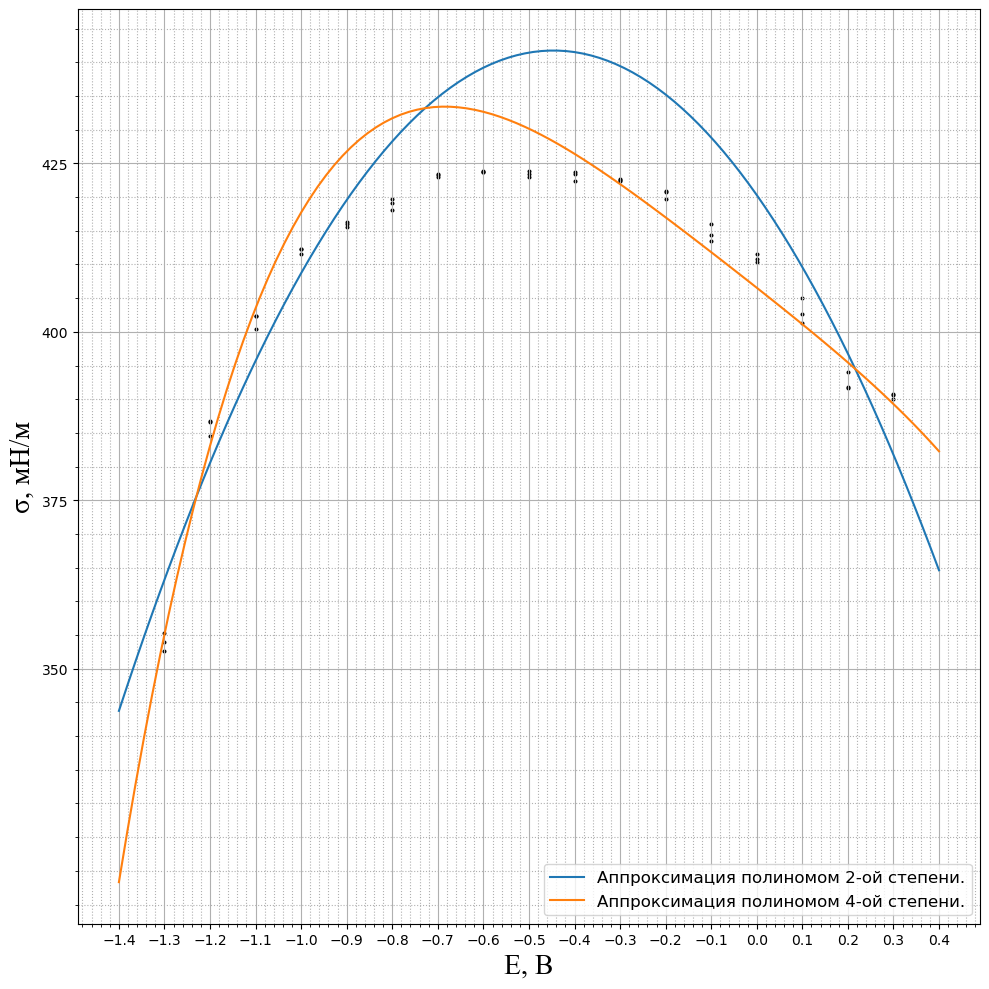
\includegraphics [scale=0.55]{Images/ЭК2.png}}
        \caption{Электрокапиллярная кривая ртутного электрода (аппроксимация далёких от ПНЗ значений.}
    \end{figure} \;
\par Вкратце приведём ниже вычисления, абсолютно аналогичные пункту 4.1.
\par Значения ПНЗ:
$$E_{2, \text{ПНЗ}} = -446,16 \; \text{мВ}$$
$$E_{4, \text{ПНЗ}} = -685,88 \; \text{мВ}$$
\par Значения электроёмкости:
$$C_{2, \text{ПНЗ}} =  21,54 \; \text{мкФ}/\text{см}^2$$
$$C_{4, \text{ПНЗ}} =  23,31 \; \text{мкФ}/\text{см}^2$$
\par Значения электроёмкости из предположения теории Штерна:
$$C_{2, \text{Г}} = 30,40 \; \text{мкФ}/\text{см}^2$$
$$C_{4, \text{Г}} = 34,05 \; \text{мкФ}/\text{см}^2$$
\par Диапазоны толщины ДЭС:
$$1,16 \; \si{\angstrom} \leq d_2 \leq 1,75 \; \si{\angstrom}$$
$$1,04 \; \si{\angstrom} \leq d_4 \leq 1,56 \; \si{\angstrom}$$
\par Таким образом, полученные значения (аппроксимация полиномом 4-ой степени хуже 2-ой степени) лучше отвечают теоретически посчитанным, что может говорить о правильном предположении, касательно аппроксимации ЭК кривой по значениям, далеким от ПНЗ. 
\end{document}
